\chapter{Artificial intelligence \& Machine Learning\label{sec:ai_and_ml}}
\par{
    Machine learning is a branch of \Gls{ai}. 
    The field of \Gls{machinevision} is a branch of machine learning.
    Some impressive steps forward have been made in the past decade, mainly thanks to the emergence of \Gls{deepl}.
}
\par{
    \Gls{ai} is showing promising results for various tasks in society.
    New research results ranging from self-driving cars to automated translation is regularly published in mainstream media.
    The aim of this chapter is not to provide a complete overview of the machine learning field.
    Instead, the objective is to highlight concepts meaningful for this work.\footnote{
        \textbf{Remark:} this work does not cover the social, legal and ethical questions \Gls{ai} evokes.
    }
    This work investigates the use of \Gls{weaklysupervisedl} data for the training and segmentation model. 
    The concept and benefits of \Gls{weaklysupervisedl} machine learning is discussed.
}

\section{Artificial Intelligence}
\par{
    The field of \Gls{ai} (AI) is the engineering discipline of the automation of \textit{cognitive} tasks.
    Tasks such as search, control and classification are generally considered to require a level of intelligence. 
    Automation of this type of tasks to allow a machine to perform them is thus \Gls{ai}\footnote{To be precise, it is not the human intelligence that is replicated. It is the \textit{effect} of this intelligence.}.
    A classic PID controller and even a thermostat controller can be viewed as simple but effective forms of AI.
    This engineering discipline has advanced considerably in the past decades, driven both by leaps forward in the available hardware and the development of new algorithms and models. 
}
\par{
    First, the availability and reliability of hardware components such as sensors, cameras, digital storage and calculation power have increased exponentially\footnote{ \textit{Moore's law} states that the number of transistors on an integrated circuit doubles every two years. This rate of progress has held more or less for a wide range of digital components in the past decades.}.
    The size and price of these components decreased equally dramatically. }
\par{
    Second, progress has been made in developing algorithms to use this available data and computation power to solve problems and perform tasks.
    This text does not provide a complete overview of all existing machine learning models. 
    This work makes use of \Gls{deepl} models.
    A \Gls{deepl} model is a type of \acrfull{ann} with multiple hidden layers. 
    Deep learning models are behind almost all recent applications of \acrfull{nlp} and \Gls{machinevision}.
}

\subsection{Neural Networks}
\todo[inline]{Illustration}
\par{
    An \acrshort{ann} is a collection of connected nodes, or \textit{neurons}. 
    These are typically structured in layers. 
    There is always an \textit{input} layer and an \textit{output} layer. Between these two, one can find the \textit{hidden} layers\footnote{When there is at least one hidden layer, one talks about a deep network. In practice, \acrshort{cnn}s have multiple hidden layers.}.
    To calculate a node value, the incoming node values are weighted by the connection weights and the result of this linear combination is transformed by an activation function\footnote{
        $\vec{x}$ : values of the nodes connected to node $j$\\
        $\vec{w}$ : connection weights\\
        $\sigma(.)$ : activation function
    }:
    \begin{eqnarray}
        z_j(\vec{x} | \vec{w}) &=& \frac{\vec{w}^T\vec{x}}{\sum w_k} \\
        y_j(\vec{x} | \vec{w}) &=& \sigma(z_j)
    \end{eqnarray}
}

\todo[inline]{Short and to-the-point introduction of convolution neural networks}
\par{
    Constructing a network requires evaluating it, comparing the evaluation output to a known desired output, and taking steps to bring the model output closer to the desired output. 
    The procedure used to fit the weights of a neural network to the 
    A network is fitted to the \textit{train set} by the optimization algorithm, based on the \textbf{loss}.
    The \acrshort{ml} engineer wants to judge the performance of the model based on one or several \textbf{metrics}, calculated on the \textit{train set}, the \textit{cross-validation set} and eventually on the \textit{test set}.
}

\subsection{Artificial intelligence for healthcare applications}

\par{
    Various researchers are exploring the opportunities of \Gls{ai} in medical practice.
    This could to reduce the burden of repetitive tasks on medical caregivers and support both medical diagnosis and procedures.
}
\par{
    \Gls{ai} applications can support medical professionals by allowing more cost effective solutions to monitors patient's condition.
    One example is the use of a \acrfull{ppg} signals to estimate a patient's blood pressure.
    Blood pressure is a valuable indicator of the patient's condition for the medical staff.
    Measuring blood pressure is time-consuming and disturbing for the patient however. 
    the \acrshort{ppg} signal is relatively easy to measure. This only requires a watch-size sensor\footnote{Several commercial sports watches already use a \acrshort{ppg} sensor to measure the athletes hear rate.} 
    around the wrist, that can be worn continuously.
    Infering the blood pressure from such a \acrshort{ppg} signal allows the healthcare worker to access valuable information continuously, cheaper and without inconvenience for the patient.
    \todo[inline]{references + ppg watch image}
}
\par{
    Different researchers investigate \Gls{machinevision} applications for medical applications. 
    Research on image classification for medical diagnosis is conducted among others for melanoma (skin cancer) diagnosis on camera (\acrshort{rgb}) images [xxx] 
    and for breast cancer diagnosis on mammographic\footnote{A mammography is an X-ray scan of the human breast.} scans [xxx].
}
\section{Machine vision}
\par{
    \Gls{machinevision} is the branch of \Gls{ai} focussed on image processing.
    The machine vision task performed in this work is called instance \Gls{segmentation}.
    This chapter explains what this means. 
    The segmentation task is compared to other machine vision tasks.
}

\subsection{Machine vision tasks \label{sec:machinevisiontasks}}
\par{
    \Gls{machinevision} is a broad discipline. 
    Humans extract information from images almost subconsciously, and we are often not aware of the different tasks we perform on images.
    The objective of this section is to briefly define different machine vision tasks discussed further in this book. 
    Several machine vision tasks consist of \textit{recognizing} objects, animals or humans in an image.
    A model is built for a finite list of \textit{categories} that can be present in an image.
    Depending on the question asked ad inference time, one can distinguish the following tasks, which are also illustrated in figure \ref{fig:machinevisiontasks}.
}
\begin{description}
    \item[Image classification] is the task of determining what object category\footnote{A slightly more advanced task is to be able to destinguish several classes in one image.} is present in the image. Is there a cat in this image?
    \item[Object counting] is the task of counting how many instances of each category are in the image. How many cats are there in this picture? 
    \item[Object detection] consists not only of identification of the object. Also, the spatial position is requested, for example in the form of a bounding box. Where is the cat in this picture if a cat is present?
    \item[Semantic segmentation] requires a class estimation for each image pixel. Pixels that do not belong to a specific class are called the \textit{background}.
    \item[Instance segmentation] requires not only that the semantic class is determined for each pixel, but also that two individuals of the same class\footnote{For each pixel, the model predicts not only if it belongs to a cat, but also which of several possible cats it belongs to.} are distinguished.   
\end{description}
\par{
    The different machine vision tasks above are ranked in order of how informative the model output is.
    It is clear that only saying if a cat is present in an image is a less informative output than indicating pixel-per-pixel where this cat is in the image.
}
\begin{SCfigure}[][h!]
    \centering
    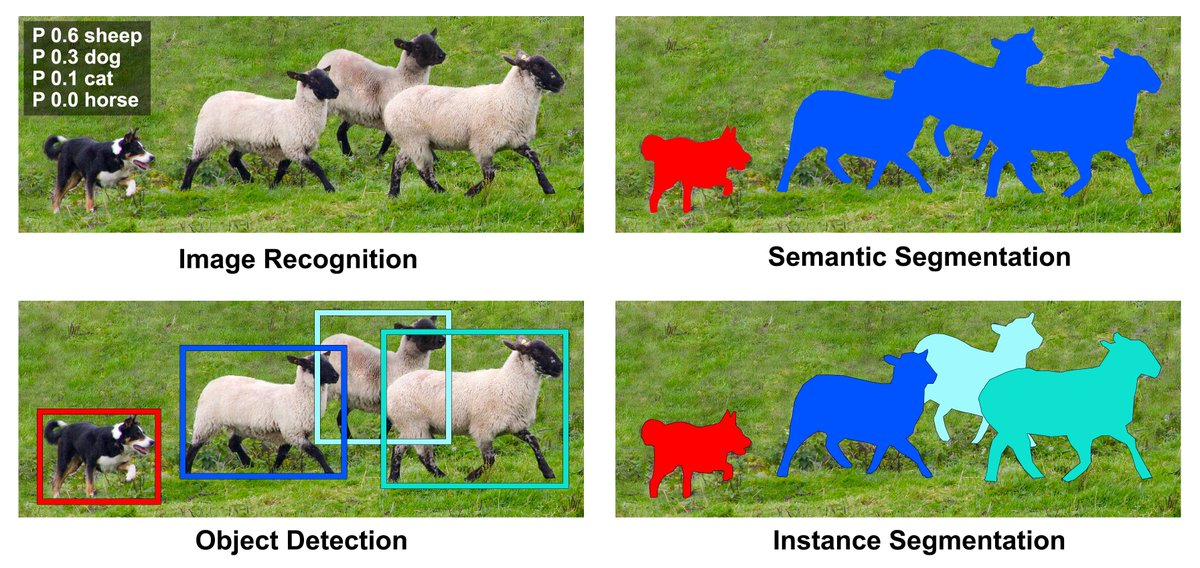
\includegraphics[width=10cm]{/home/thesis/images/Classification_vs_Segmentation.jpg}
    \caption{Illustration to compare different Machine vision tasks \cite{SemTorch76:online}. 
    Object detection means that the location of several objects is estimated by the model. This is indicated by the \textit{bounding boxes}.
    Segmentation of an image is classifying each pixel in the correct class or assigning it to the \textit{background} class.
    Semantic segmentation makes no difference between different instances of the same semantic class, instance segmentation does.
    \label{fig:machinevisiontasks}}
\end{SCfigure}


\subsection{The convolution layer}

The building block of virtually every modern machine vision network, including the ones in this thesis, is the convolution layer.

\todo[inline]{weight sharing, feature extraction}

\subsection{Data for training machine vision models}
\par{
    To perform the tasks discussed in chapter \ref{sec:machinevisiontasks}, one needs to build a suitable model.
    For \Gls{machinevision} tasks\footnote{and many other tasks.}, the current standard approach is \Gls{deepl}.
    The cost to generate, store and communicate images and computation power has dropped in the past decades.
    This evolution allows to train a model  on previously unimaginable quantities of data\footnote{The \textit{ImageNet} database (\url{http://image-net.org/challenges/LSVRC/index}) consists of more than $14.10^6$ images.}.
    This technique allows a model with a high number of degrees of freedom to be trainded\footnote{learn by example, so you will} without the need for expert-crafted features. 
}
\subsubsection{Weak supervision types\label{sec:weak_supervision}}
\par{
    To build a model to perform the tasks discussed in \ref{sec:machinevisiontasks}, this model needs to be trained.
    This requires a set of \textit{labelled} images.
    Collection of this dataset - most importantly, the labels - proves to be a challenge. 
    Training a model with \textit{weak labels} compared to \textit{strong labels} could help to mitigate the labelling cost problem.
}
\par{
    In the classic approach, the supervision type closely resembles the intended model output.
    To train a model that can classify an image\footnote{Given an image, the model outputs if this picture is a representation of class \textit{cat}, \textit{dog} or another animal or object. }, 
    one has to \textit{train} the model on a set of labelled images where a human indicated the class.
    To train a model to perform image segmentation\footnote{segmentation means that the model classifies each pixel.}, an expert needs to provide a set of images in which each picture, the objects are delineated.  
}
\par{
    In the classic approach, the data labels closely resemble the output sought to obtain from the model.
    The idea behind \Gls{weaklysupervisedl} is to train a model with cheaper annotations that contain less information than the desired model output, making use of the latent information available in the labels without explicitly indication.
    Figure \ref{fig:ImageLabelTypes} illustrates several types of image supervision : 
    From left to right on the top row, this shows point supervision and squiggle annotation, common annotation types for weak supervision.
    On the second row, bounding box annotation and complete mask annotation are illustrated.
}

\begin{SCfigure}[][htb]
    \centering
    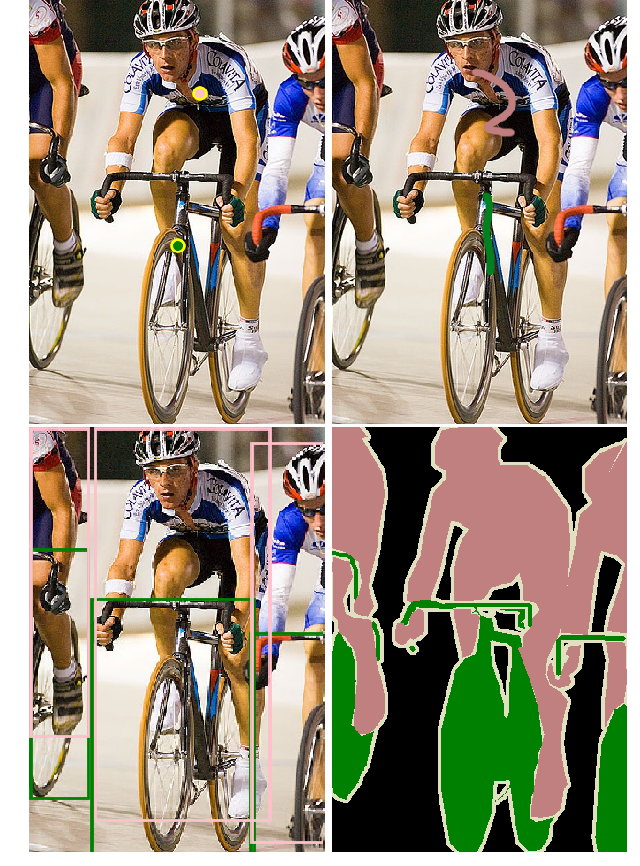
\includegraphics[width=10cm]{/home/thesis/images/McEver.png}
    \caption{Four different annotation types \cite{McEver2020}: 
    On the top left the picture is point level annotated. The points are inflated for visibility.
    On the top right, squiggle annotation is used.
    The bottom left shows bounding box supervion.
    While the bottom right image is fully annotated.
    An image level label would indicate that there are multiple instances of \textit{person} and \textit{bike} in the image.
    \label{fig:ImageLabelTypes}}
\end{SCfigure}

\par{
    The objective of \Gls{weaklysupervisedl} is to construct a robust model based on \textit{cheap} (incomplete, noisy or imprecise) labels, sometimes described as \textit{indirect supervision}.
    Numerous creative approaches have been conceived.
    Since the provided annotations in \Gls{weaklysupervisedl} are not full labels, these are sometimes described as \textit{hints} instead
    %\footnote{
    %    This is based on the insightfull talk at \url{ 
    %        https://youtu.be/4EjYxVVCAaE
    %    }. For example, the destinction between labels and hints.
    %}.
    The basic concept of \Gls{weaklysupervisedl} is that there are two sources of information to draw from: The hints and the prior knowledge about the problem (Priors).
    These \textit{Priors} can be any form of prior knowledge about the object to be segmented\footnote{or any other machine vision task.}.
    Priors can be the object size, shape or location, the number of instances, the similarity across images or the similarity with external images.
}
\par{
    Whether an annotation is considered a \textit{weak label} or a \textit{strong label} depends more on the modeller's intention than on the annotation itself. 
    When one aims to construct a model to infer output labels with a higher informative value than the original annotations, these \textit{labels} become \textit{hints}.
    Making a model predict bounding boxes from a dataset annotated with bounding boxes means considering these as \textit{strong labels}. 
    If one uses the same dataset to construct a model that predicts pixel-wise masks, the labels are \textit{weak labels} or \textit{hints}.
}


For a segmentation task, weak labels can be:
\begin{description}
    \item[Image level labels]: In this case, only the object class of the object in the image is provided. 
    This would be a full label for a classification task, but it is a weak label for a segmentation task\footnote{Image with image level annotation can, for some problems, be obtained in large numbers by web-scraping.}.
    \item[Point annotation]: This annotation technique, the subject of this work, consists of asking the expert to indicate the classes with one or several points. This technique is used in \cite{Laradji2020, Laradji2018, McEver2020}.
    In \cite{Mainis}, instead of \textit{random} point annotation, the author makes use of \textit{extreme} point annotation.  
    \item[Squiggles]: This annotation technique is related to the point annotation technique. Instead of points, the expert is asked to indicate the classes with a squiggly line.
    \item[Bounding boxes]: A bounding box (a rectangle circumscribing the object) is a less precise form of object localization than pixel-wise segmentation.
    \item[Image description]: This task combines the problem of \acrlong{nlp} with the problem of image segmentation. The annotation of the image is derived from verbal or written description of the image. 
    This annotation type has not yet been used by many researchers. 
    It might be promising since large bodies of datasets could be available from for example medical files where a medical expert has provided a written diagnosis based on available medical images. 
\end{description}
\par{
    There seem to be endless variations possible to conceive weak labels. 
    For example, instead of image level labels, in \cite{Laradji2018}, the number of instances of the specific class\footnote{Which happens to be pinguins.} is provided. 
}
\par{
    In \cite{Bearman2015}, Bearman et al. compare the annotation time required for images from the PASCAL VOC 2012 dataset.
    The authors report an average time per image of 239.7 seconds per image for full image pixel annotation, 20.0 seconds per image for image level labels and 22.1 seconds per image for point annotation.
    As is repeated in \ref{sec:PreviousWork_weaklySupervised}, point lavel annotation is attractive since it barely requires more of the expert's time while delivering more precise information.
    The point label contains valuable localization information, absent from the image level annotation.
}
\\[5pt]
\par{
    Many techniques to train models on weakly supervised data are more computationaly intensive than techniques to train models on fully supervised data.
    The loss functions itself consist of multiple parts and might involve repeated evaluation of the model on the same batch. 
    A two step process sometimes used where a first model generates pseudo masks to train a second model on these pseudo mask as if it were a fully supervised task.
    Weakly supervised learning is based on the idea that the cost of human experts is fixed, or even increasing while the cost of computation power is decreasing.
    Besides this, the ability to label more data at the same labelling price point can increase the variability of the data the model is trained on. 
    This can increase the robustness of the model.
}